\chapter{Results}

Dans ce chapitre, nous présontons les résultats de la méthode exposée préscédemment. 

3.1. Sensor Space : Nous commonçons par étudier la donnée dans le time-frequency space afin de trouver les temps et les frequences les plus importantes:
- La classification par CSP nous a permis d'obtenir une time-frequency map qui permet d'associer à chaque temps et frequences une roc auc. Cette roc auc indique à quel point l'information stoquée dans la mémoire de travail est décodable par des informations géométrique.
- Les statisitques par permutation permettent de vérifier la significativité du time-frequency cluster obtenu.

3.2. Source space. Apres avoir vérifié la significativité statistique de notre cluster, nous utilisons ce cluster pour projeter l'information dans un espace tridimensionel, (aka l'espace des sources), afin d'y visualiser le contraste entre la mémoire de travail chargée avec 3-items contre 1-item. C'esr principalement cette étape qui permet d'extraire les informations neuroanatomiques.

\section{Sensor space results}

\subsection{CSP results}


\begin{figure}
    \centering
    \begin{subfigure}{.5\textwidth}
        \centering
        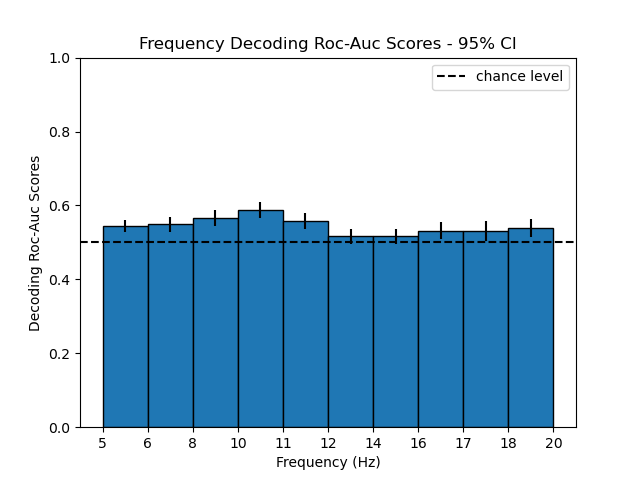
\includegraphics[width=1.\linewidth]{images_report/sensor/csp_permutation_res/csp_frequency.png}
        \caption{CSP frequency decoding.}
        \label{fig:csp_frequency}
    \end{subfigure}%
    \begin{subfigure}{.5\textwidth}
        \centering
        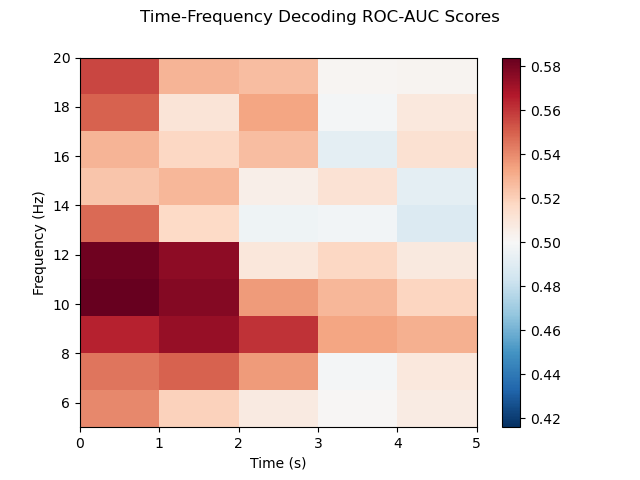
\includegraphics[width=1.\linewidth]{images_report/sensor/csp_permutation_res/csp_time_frequency.png}
        \caption{CSP time-frequency decoding.}
        \label{fig:csp_time_frequency}
    \end{subfigure}
    \caption{CSP results for the average subject.}
    \label{fig:csp_results}
\end{figure}


% [expliquer avant que le csp est appliqué pour différentes bins et que l'on compare par la suite le roc auc score pour différentess bins, ce qui permet de mettre les régions d'interet en ]

In the figure \ref{fig:csp_results}, we observe the roc-auc score of the classifier composed of (CSP, logistic regression) for different frequencies distributed linearly between 5 Hz and 20 Hz as well as for times between $t=0$ and $t=5$ seconds (the figures \ref{fig:Evoked_data}, \ref{fig:decoding_initial} presented the times $t \leq 0$ only for pedagogical purposes). We can see that the CSP algorithm succeeded in highlighting the alpha frequency band between 8 and 12 Hz, and the results are consistent between the frequency map \ref{fig:csp_frequency} and the time-frequency map \ref{fig:csp_time_frequency}.

\subsection{Cluster Permutation Test results}

\begin{figure}[ht]
    \centering
    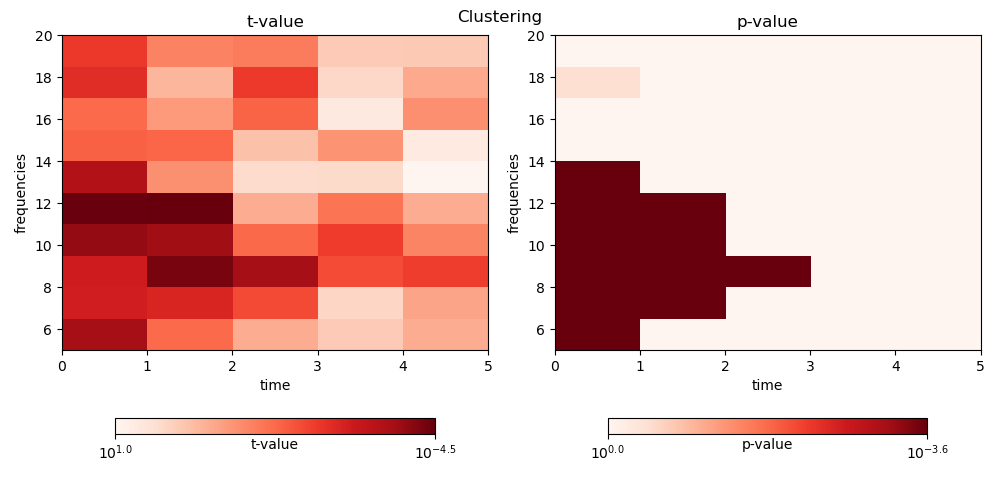
\includegraphics[width=15cm]{images_report/sensor/csp_permutation_res/permutations_test.png}
    \caption[Permutation statistics results.]%
    {Permutation statistics results.}
    \label{permutation_statistics_results}
\end{figure}

\section{Sensor results discussion}

\paragraph{Quantitative analysis}
An AUC of 0.6 is not high in absolute terms but not bad in neuroscience on intervals of only 0.5 seconds. If we combine all the bins we would get a much better AUC. Furthermore, statictics by permutation of clusters show that the results are very significant at the group level.

\paragraph{Qualitative analysis}

Our main cluster is centered on the alpha band. We will discuss the alpha band in more detail in section \ref{section:alpha_discussion}. But at first sight, the literature shows frequently significant results in the alpha band for working memory loadings \cite{obleser2012adverse} which is encouraging.

A surprising phenomenon is that the algorithm can decode much more easily at the beginning of the restitution phase than at the end of the restitution phase. Given that the csp encodes a geometric information, this means that:
\begin{itemize}
    \item either the information in the working memory is transformed in the course of restitution into information disseminated in the brain in a non-geometrical way.
    \item Or, given the very large number of repetitions of the experiment, the subject gets tired after a while and forgets the sequence "instantly" after having repreated it in order to save mental energy.
\end{itemize}



\section{Results of the contrast in source space²}


\begin{figure}[ht]
    \centering
    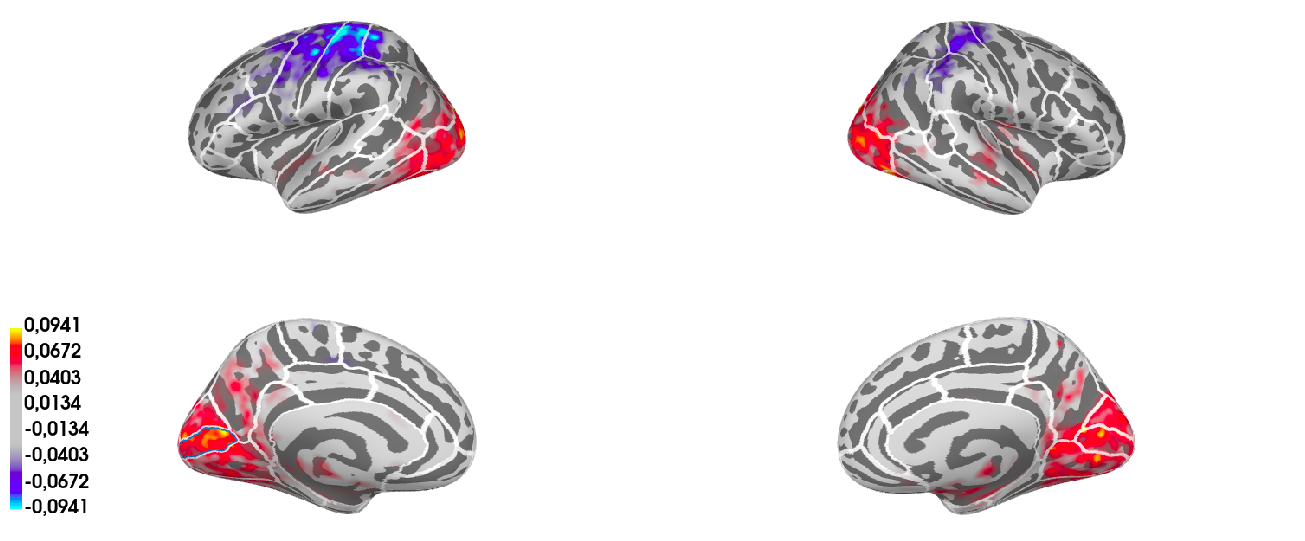
\includegraphics[width=15cm]{images_report/source/source_results_3d_cropped.png}
    \caption[Contrast results in the source space (alpha)]%
    {Contrast results in source space for 0s-1s, and 8Hz-14Hz (alpha).}
    \label{results_source_space_alpha}
\end{figure}

\begin{figure}[ht]
    \centering
    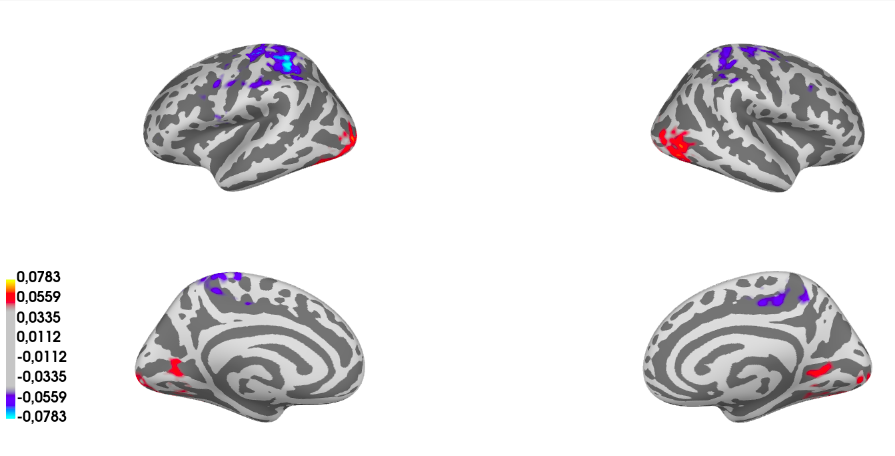
\includegraphics[width=13cm]{images_report/source/source_results_beta_1s.png}
    \caption[Results of the contrast in the source space.]%
    {Contrast results in source space for 0s-1s, and 15Hz-20Hz (beta).}
    \label{results_source_space_beta}
\end{figure}
 
The figure \ref{results_source_space_alpha} presents the results of the contrast in source space for the most significant time-frequency bin at the group level, i.e. 0s-1s, and 8Hz-14Hz. In this figure the red regions are the regions activated for 3 items, while the blue regions are more activated for 1 item. We recall that 3 items are supposed to load the working memory more than 1 item.

\paragraph{Occipital cortex (visual)}
\label{section:alpha_discussion}
The red region activated here is the visual area. The fact that we see the visual area here is not surprising. Indeed, we have to remember that we are visualizing here the alpha band which is a classically inhibitory band in the tlitterature. Thus, the classical interpretation of an activation in the alpha band corresponds to an inhibition of the function of the associated region. This is confirmed by the fact that when we look at the activation in the beta \ref{results_source_space_beta} of our contrast, the activation of the visual cortex (the red region) disappears almost completely.

The literature presents other results similar to this one. For example \cite{obleser2012adverse} shows that "Enhanced alpha oscillations (8-13 Hz) during retention of items in working memory are often interpreted to reflect increased demands on storage and inhibition".

\paragraph{Sensori-Motor Areas}

\begin{figure}[ht]
    \centering
    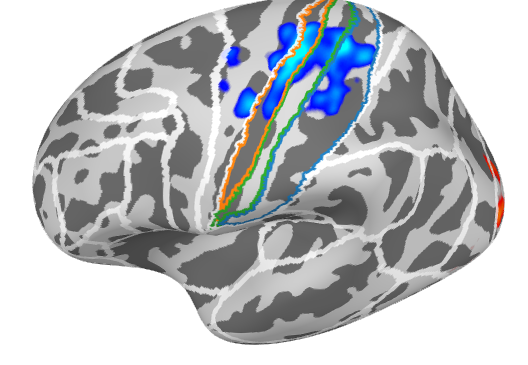
\includegraphics[width=7cm]{images_report/source/brodmann_alpha.png}
    \caption[Focus on the Brodmann areas]%
    {Focus on the Brodmann areas 1 (green), 2 (blue) and 3 (orange), from the alpha band in the left hemisphere.}
    \label{brodmann_alpha}
\end{figure}

The blue region activated at the top of the brain is the sensori-motor area, centred on the postcentral gyrus (Brodmann areas 1, 2 and 3). Before the MEG experiment, subjects were trained to reproduce the task by pressing a button, which explains the activation here. And the region of the somatosensory cortex activated here corresponds to the location of the hand receptors \ref{brodmann_alpha}. This is also supported by the fact that the activation is stronger in the left hemisphere which is consistent with the fact that the subjects are right-handed.

A possible interpretation is that time is represented by the imagination of the movement of one of the body parts, here the hand. We can also reason by analogy by noting that musical children learn to master rhythms by beating the beat or walking to the rhythm of the pulse. The rhythmic information is embodied. Therefore, even if here the analogy has limits since the temporal signal is not organized in a rhythmic and regular way, this interpretation seems to us to be the most natural one.

\paragraph{Auditory area}

The regions close to the ears are deactivated while the cue is an auditory one. There are several interpretations:
- To see an activation in the auditory zones one must place oneself at $t \leq 0$, as on the figures \ref{auditory_cortex}: After $t \geq 0$, the auditory cortex is no longer involved
- The signal is abstracted from the auditory region to transform it into a purely rhythmic information, thus no longer restricted to the auditory areas.
- The auditory region is activated, but we do not see it in this group figure. As a matter of fact, the auditory regions are visible in the csp components of the subjects as in the figure \ref{fig:csp_component_beta_band}. But there is a lot of inter-subject variability: After looking at the csp components for the different subjects, it appears that only subjects with a marked beta peak show activation in auditory cortex, and this peak is not restricted to $0 \leq t \leq 1$ but are spread across all subjects between $0s - 5s$. In order to see an auditory signal at the group level, one would have to align and average the first extracted components for each peak from each subject. But averaging the components presents mathematical difficulties [ref. Appendix], and could be a research topic in itself.

[Image beta et pour csp aussi.]

% \section{Discussion}

% encore un résumé